% THIS DOCUMENT IS TAILORED TO REQUIREMENTS FOR SCIENTIFIC COMPUTING.  IT SHOULDN'T
% BE USED FOR NON-SCIENTIFIC COMPUTING PROJECTS
\documentclass[12pt]{article}

\usepackage{amsmath, mathtools}
\usepackage{amsfonts}
\usepackage{amssymb}
\usepackage{graphicx}
\usepackage{colortbl}
\usepackage{xr}
\usepackage{hyperref}
\usepackage{longtable}
\usepackage{xfrac}
\usepackage{tabularx}
\usepackage{float}
\usepackage{siunitx}
\usepackage{booktabs}
\usepackage{caption}
\usepackage{pdflscape}
\usepackage{afterpage}

\usepackage[round]{natbib}

%\usepackage{refcheck}

\hypersetup{
    bookmarks=true,         % show bookmarks bar?
      colorlinks=true,       % false: boxed links; true: colored links
    linkcolor=red,          % color of internal links (change box color with linkbordercolor)
    citecolor=green,        % color of links to bibliography
    filecolor=magenta,      % color of file links
    urlcolor=cyan           % color of external links
}

\input{../Comments}
\input{../Common}
%\input{Comments}
%\input{Common}

% For easy change of table widths
\newcommand{\colZwidth}{1.0\textwidth}
\newcommand{\colAwidth}{0.13\textwidth}
\newcommand{\colBwidth}{0.82\textwidth}
\newcommand{\colCwidth}{0.1\textwidth}
\newcommand{\colDwidth}{0.05\textwidth}
\newcommand{\colEwidth}{0.8\textwidth}
\newcommand{\colFwidth}{0.17\textwidth}
\newcommand{\colGwidth}{0.5\textwidth}
\newcommand{\colHwidth}{0.28\textwidth}

% Used so that cross-references have a meaningful prefix
\newcounter{defnum} %Definition Number
\newcommand{\dthedefnum}{GD\thedefnum}
\newcommand{\dref}[1]{GD\ref{#1}}
\newcounter{datadefnum} %Datadefinition Number
\newcommand{\ddthedatadefnum}{DD\thedatadefnum}
\newcommand{\ddref}[1]{DD\ref{#1}}
\newcounter{theorynum} %Theory Number
\newcommand{\tthetheorynum}{TM\thetheorynum}
\newcommand{\tref}[1]{TM\ref{#1}}
\newcounter{tablenum} %Table Number
\newcommand{\tbthetablenum}{TB\thetablenum}
\newcommand{\tbref}[1]{TB\ref{#1}}
\newcounter{assumpnum} %Assumption Number
\newcommand{\atheassumpnum}{A\theassumpnum}
\newcommand{\aref}[1]{A\ref{#1}}
\newcounter{goalnum} %Goal Number
\newcommand{\gthegoalnum}{GS\thegoalnum}
\newcommand{\gsref}[1]{GS\ref{#1}}
\newcounter{instnum} %Instance Number
\newcommand{\itheinstnum}{IM\theinstnum}
\newcommand{\iref}[1]{IM\ref{#1}}
\newcounter{reqnum} %Requirement Number
\newcommand{\rthereqnum}{R\thereqnum}
\newcommand{\rref}[1]{R\ref{#1}}
\newcounter{nfrnum} %NFR Number
\newcommand{\rthenfrnum}{NFR\thenfrnum}
\newcommand{\nfrref}[1]{NFR\ref{#1}}
\newcounter{lcnum} %Likely change number
\newcommand{\lthelcnum}{LC\thelcnum}
\newcommand{\lcref}[1]{LC\ref{#1}}

\usepackage{fullpage}

\newcommand{\deftheory}[9][Not Applicable]
{
\newpage
\noindent \rule{\textwidth}{0.5mm}

\paragraph{RefName: } \textbf{#2} \phantomsection 
\label{#2}

\paragraph{Label:} #3

\noindent \rule{\textwidth}{0.5mm}

\paragraph{Equation:}

#4

\paragraph{Description:}

#5

\paragraph{Notes:}

#6

\paragraph{Source:}

#7

\paragraph{Ref.\ By:}

#8

\paragraph{Preconditions for \hyperref[#2]{#2}:}
\label{#2_precond}

#9

\paragraph{Derivation for \hyperref[#2]{#2}:}
\label{#2_deriv}

#1

\noindent \rule{\textwidth}{0.5mm}

}

\begin{document}

\title{Software Requirements Specification for Re-ProtGNN: Re-implementation of the ProtGNN model} 
\author{\authname}
\date{\today}
	
\maketitle

~\newpage

\pagenumbering{roman}

\tableofcontents

~\newpage

\section*{Revision History}

\begin{tabularx}{\textwidth}{p{3cm}p{2cm}X}
\toprule {\bf Date} & {\bf Version} & {\bf Notes}\\
\midrule
Feb 6, 2024 & 1.0 & First Draft\\
\bottomrule
\end{tabularx}

~\\

~\newpage

\section{Reference Material}

This section records information for easy reference.

\subsection{Table of Units}
Not applicable, as there is no unit in this software.

\subsection{Table of Symbols}

The table that follows summarizes the symbols used in this document along with
their units.  The choice of symbols was made to be consistent with the heat
transfer literature and with existing documentation for solar water heating
systems.  The symbols are listed in alphabetical order.

\renewcommand{\arraystretch}{1.2}
\noindent \begin{longtable*}{l l p{12cm}} \toprule
\textbf{symbol} & \textbf{unit} & \textbf{description} \\
\midrule 
$X$ & Unitless & Node feature matrix \\
$X_p$ & Unitless & Prototype node feature matrix \\
$A$ & Unitless & Adjacency matrix \\
$A_p$ & Unitless & Prototype adjacency matrix \\
$y$ & Unitless & True class label \\
$\hat{y}$ & Unitless & Predicted class label \\
$W$ & Unitless & Weight matrix for the fully connected layer \\
$b$ & Unitless & Bias term \\
$W_g$ & Unitless & Weight matrix for GNN encoder \\
$P$ & Unitless & Prototype representations \\
$h$ & Unitless & Graph embedding \\
$\sigma$ & Unitless & Sigmoid activation function \\
$\mathcal{L}$ & Unitless & Loss function \\
$L_{CE}$ & Unitless & Cross-entropy loss \\
$L_{Clst}$ & Unitless & Cluster loss \\
$L_{Sep}$ & Unitless & Separation loss \\
$L_{Div}$ & Unitless & Diversity loss \\
$\eta$ & Unitless & Learning rate \\
$\lambda_1, \lambda_2, \lambda_3$ & Unitless & Regularization parameters \\
$h_v^{k+1}$ & Unitless & Node representation at layer $k+1$ \\
$h_u^k$ & Unitless & Representation vector of node $u$ at layer $k$ \\
$\tilde{A}$ & Unitless & Normalized adjacency matrix \\
$\hat{A}$ & Unitless & Adjacency matrix with self-connections \\
$\hat{D}$ & Unitless & Diagonal degree matrix where $\hat{D}_{ii} = \sum_j \hat{A}_{ij}$ \\
$W^k$ & Unitless & Trainable weight matrix at layer $k$ \\
$\mathcal{N}(v)$ & Unitless & Neighborhood of node $v$, i.e., set of adjacent nodes \\
$s_{\max}$ & Unitless & Cosine similarity threshold for prototype diversity loss \\
$C$ & Unitless & Number of classes in the classification task \\
\bottomrule
\end{longtable*}


\subsection{Abbreviations and Acronyms}

\renewcommand{\arraystretch}{1.2}
\begin{tabular}{l l} 
  \toprule		
  \textbf{symbol} & \textbf{description}\\
  \midrule 
  A & Assumption\\
  DD & Data Definition\\
  GD & General Definition\\
  GS & Goal Statement\\
  IM & Instance Model\\
  LC & Likely Change\\
  PS & Physical System Description\\
  R & Requirement\\
  SRS & Software Requirements Specification\\
  TM & Theoretical Model\\
  ProtGNN & Prototype-based Graph Neural Network\\
  Re-ProtGNN & Re-implementation of the ProtGNN model\\
  GNN & Graph Neural Network\\
  GCN & Graph Convolutional Network\\
  GIN & Graph Isomorphism Network\\
  \bottomrule
\end{tabular}\\


\subsection{Mathematical Notation}

\renewcommand{\arraystretch}{1.2}
\noindent \begin{longtable*}{l p{7cm} l} 
\toprule
\textbf{Notation} & \textbf{Description} & \textbf{Source} \\
\midrule 
$num\_rows(\cdot)$ & Number of rows in a matrix & - \\
$num\_cols(\cdot)$ & Number of columns in a matrix & -\\
$\dim(\cdot)$ & Dimension of a matrix & - \\
$M[i, j]$ & Element at row $i$, column $j$ in matrix $M$ & - \\
$f(\cdot)$ & A function representing the graph encoder, as defined in \tref{TM1:GNNFP} & - \\
$\cos(\cdot, \cdot)$ & Cosine similarity function & ~\citep{sciencedirect_cosine_similarity} \\
$\text{ReLU}(\cdot)$ & ReLU activation function & ~\citep{wikipedia_relu} \\
$\nabla$ & Gradient operator & ~\citep{wikipedia_gradient} \\
\bottomrule
\end{longtable*}




\section{Introduction}

Graph Neural Networks (GNNs) have shown strong performance in node classifi-
cation, graph classification, and link prediction tasks. However, their black-box
nature makes it difficult to understand their decision-making process, limiting
their usage in critical areas such as medical diagnosis. 

To address this, the paper \textit{ProtGNN: Towards Self-Explaining Graph Neural Networks} ~\citep{zhang2022} proposes ProtGNN (Prototype-based Graph Neural Network), an interpretable GNN model designed to improve explainability by learning representative prototypes for each class. The goal of this project is to re-implement ProtGNN and validate its results. Further details on the problem and motivation behind this project can be found in the Problem Statement document~\citep{yuanqi2025protgnn}.

The introduction section outlines the Software Requirement Specifications (SRS) for Re-ProtGNN (Re-implementation of the ProtGNN model), detailing its purpose, scope, target audience, and organization.

\subsection{Purpose of Document}
The purpose of this SRS document is to define and communicate the requirements, constraints, and models for the Re-ProtGNN project. It serves as a formal reference and links to the other documents of this project.


\subsection{Scope of Requirements} 
Re-ProtGNN is a re-implementation of the existing ProtGNN model, aimed at reproducing its results and validating its performance on graph datasets. The model operates in a supervised setting, performing graph classification while incorporating built-in interpretability. 

The input graphs for training must be valid labeled graphs, ensuring they contain both structural and node feature information necessary for classification. Further details on data constraints and assumptions can be found in (Section~\ref{sec_assumpt}).


\subsection{Characteristics of Intended Reader} \label{sec_IntendedReader}

This document is intended for machine learning researchers, AI practitioners, and students who are interested in interpretable GNNs and prototype-based learning. To effectively understand and utilize this document, the reader should have:
\begin{itemize}
    \item High-school knowledge of calculus, particularly partial derivatives and gradient-based optimization.
    \item Completion of an undergrad-level course or equivalent experience in
supervised learning (e.g., logistic regression) and
neural networks (including backpropagation, loss functions, and optimization).
    \item Familiarity with graph-based learning (e.g., message-passing mechanisms in GNNs) is recommended but not required.
    \item Experience with Python and PyTorch, including implementing and training neural networks.
    \item Basic knowledge of model explainability in AI, including the concept of prototypes in classification models.
\end{itemize}

This document is designed to be accessible to readers with the above qualifications. However, researchers with limited exposure to graph neural networks can still benefit from the explanations provided, as long as they have a strong foundation in deep learning and optimization methods.

\subsection{Organization of Document}

This SRS document is based on the template by ~\citep{SmithAndLai2005, SmithEtAl2007}. It systematically presents the system's objectives, theoretical foundations, assumptions, and models. For a structured reading approach, readers may start with the goal statements (Section~\ref{sec_goals}), followed by the theoretical models (Section~\ref{sec_theoretical}) and general definitions (Section~\ref{sec_gendef}), which build upon these goals. The document concludes with instance models (Section~\ref{sec_instance}), providing a concrete understanding of the system’s actual implementation.

\section{General System Description}

This section provides general information about the system.  It identifies the
interfaces between the system and its environment, describes the user
characteristics and lists the system constraints.

\subsection{System Context}


\begin{figure}[h!]
\begin{center}
 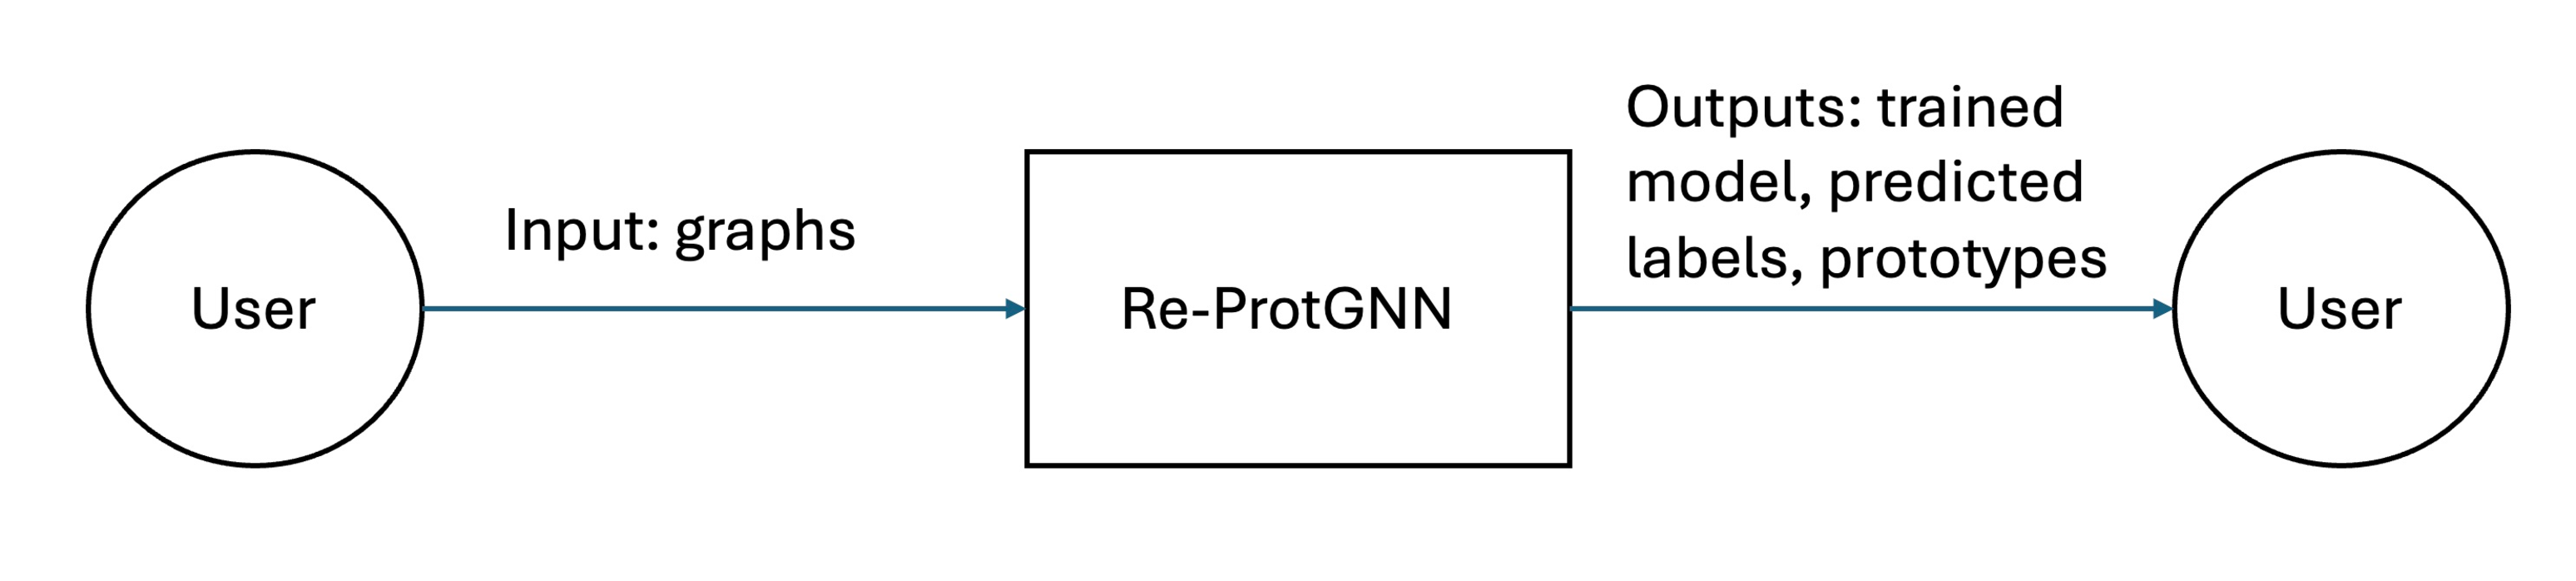
\includegraphics[width=0.9\textwidth]{SystemContextFigure}
\caption{System Context}
\label{Fig_SystemContext} 
\end{center}
\end{figure}

\begin{itemize}
\item User Responsibilities:
\begin{itemize}
\item Download the MUTAG dataset and load it to Re-ProtGNN. 
\item Run Re-ProtGNN on a system with appropriate computational resources.
\item Interpret the model’s output, including classifications and prototype-based explanations.
\end{itemize}
\item Re-ProtGNN Responsibilities:
\begin{itemize}
\item Train a GNN model using gradient-based optimization.
\item Provide classification predictions.
\item Learn prototype representations.
\item Offer visualization tools for understanding learned prototypes.
\end{itemize}
\end{itemize}

\subsection{User Characteristics} \label{SecUserCharacteristics}

The end user of Re-ProtGNN includes anyone working with GNNs or those interested in interpretable deep learning models. While prior experience with interpretable machine learning is beneficial, it is not required. The basic skill set needed to use Re-ProtGNN includes basic computer literacy and a high school-level understanding of graphs.




\subsection{System Constraints}

The Re-ProtGNN system has the constraints that the input must be a valid graph dataset (i.e., adjacency matrices, node features).

\section{Specific System Description}

This section first presents the problem description, which gives a high-level
view of the problem to be solved.  This is followed by the solution characteristics
specification, which presents the assumptions, theories, definitions and finally
the instance models.

\subsection{Problem Description} \label{Sec_pd}
Traditional GNNs excel in graph classification tasks but function as black-box models, making it difficult for users to understand their classification decisions. ProtGNN addresses this lack of interpretability by incorporating prototype-based explanations into graph classification. This project, Re-ProtGNN, is a re-implementation of ProtGNN, aimed at validating its reproducibility and performance on benchmark datasets.


\subsubsection{Terminology and  Definitions}

This subsection provides a list of terms that are used in the subsequent
sections and their meaning, with the purpose of reducing ambiguity and making it
easier to correctly understand the requirements:

\begin{itemize}

\item Graph: A structure consisting of nodes and edges, typically represented by a node feature matrix and an adjacency matrix.
\item Graph Classification: The task of assigning a label to an entire graph based on its structure and node attributes.
\item Graph Neural Networks: A type of deep learning model designed to process graph-structured data by aggregating and transforming node information.
\item Prototype: A representative subgraph that highlights the key structural patterns influencing classification decisions.
\item MUTAG Dataset: A benchmark dataset for molecular graph classification, distinguishing between mutagenic and non-mutagenic compounds ~\citep{debnath1991structure}.
\item Supervised Learning: A training approach where the model learns from labeled data, mapping input graphs to their corresponding class labels.

\end{itemize}

\subsubsection{Physical System Description} \label{sec_phySystDescrip}

The physical system of Re-ProtGNN, as shown in Figure ~\ref{PS_Figure},
includes the following elements:

\begin{itemize}

    \item[PS1:] Graph Inputs: The dataset consists of labeled graphs used for graph classification (e.g., MUTAG).

    \item[PS2:] GNN Encoder: A GNN-based encoder (e.g., GCN, GIN) extracts node and graph-level embeddings through message passing. Graph embeddings are used for both classification and prototype learning.

    \item[PS3:] Prototype Layer: A prototype layer learns representative subgraph embeddings that characterize structural patterns of different classes. Prototypes are updated during training to match key graph structures associated with class labels.

    \item[PS4:] Fully Connected Layer: The model classifies graphs based on their learned representations. The most similar prototype is retrieved to justify the classification result.

    \item[PS5:] Training Process: The model is trained using supervised learning, optimizing a combined cross-entropy loss and prototype-based losses.

    \item[PS6:] Inference Process: The trained model classifies new graphs and provides prototype-based explanations. Prototype similarity scores are used to explain classification decisions.

\end{itemize}


\begin{figure}[h!]
\begin{center}
% %\rotatebox{-90}
{
  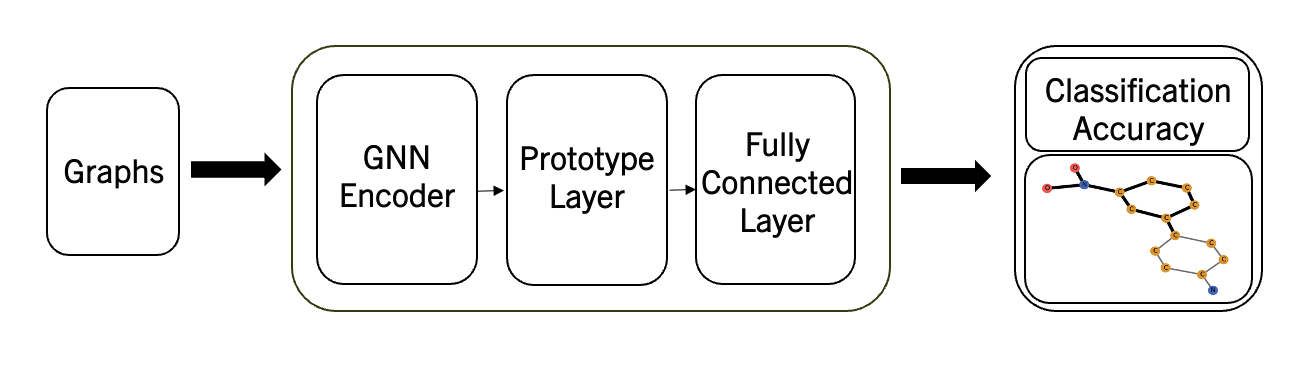
\includegraphics[width=1\textwidth]{PhysicalSystem.png}
 }
     \caption{\label{PS_Figure} The ProtGNN Framework}
 \end{center}
 \end{figure}

\subsubsection{Goal Statements} \label{sec_goals}

\noindent Given the input graphs, the goal statement is:

\begin{itemize}

\item[GS\refstepcounter{goalnum}\thegoalnum \label{GS1}:] Output a trained model that classifies the input graphs and identifies a few prototypes (i.e., key graph structures that contribute to classification) for each class.

\end{itemize}

\subsection{Solution Characteristics Specification}

The instance models that govern Re-ProtGNN are presented in
Subsection~\ref{sec_instance}.  The information to understand the meaning of the
instance models and their derivation is also presented, so that the instance
models can be verified.

\subsubsection{Types}

\begin{tabular}{l l} 
  \toprule		
  \textbf{symbol} & \textbf{description}\\
  \midrule 
  $\mathbb{Z}$ & Integer\\
  $\mathbb{R}$ & Real number\\
  \bottomrule
\end{tabular}\\

\subsection{Scope Decisions} \label{sec_scopeDec}
Re-ProtGNN focuses on validating the classification accuracy and prototype quality of the ProtGNN model using the MUTAG dataset~\citep{debnath1991structure}.


\subsubsection{Modelling Decisions}
Re-ProtGNN follows the same model design and has the same Loss Function (see \iref{TM2:LF}) as ProtGNN.

\subsubsection{Assumptions} \label{sec_assumpt}

This section simplifies the original problem and helps in developing the
theoretical model by filling in the missing information for the physical system.
The numbers given in the square brackets refer to the theoretical model [TM],
general definition [GD], data definition [DD], instance model [IM], or likely
change [LC], in which the respective assumption is used.

\begin{itemize}

\item[A\refstepcounter{assumpnum}\theassumpnum \label{A1}:]
  The node features of input graphs are relevant to classification, as required by \tref{TM1:GNNFP} to produce meaningful graph embeddings.

\item[A\refstepcounter{assumpnum}\theassumpnum \label{A2}:]
  The structural patterns of input graphs are relevant to classification, as required by \tref{TM1:GNNFP} to produce meaningful graph embeddings.

\item[A\refstepcounter{assumpnum}\theassumpnum \label{A3}:]
    For the training phase \iref{Training} to produce an accurate model and the inference phase \iref{Inference} to generate reasonable predictions and prototypes, each input graph must belong to one of the two predefined classes (i.e., mutagenic or non-mutagenic) as defined in the MUTAG dataset~\citep{debnath1991structure}.

    
\end{itemize}

\subsubsection{Theoretical Models}\label{sec_theoretical}

This section focuses on the general equations and laws that Re-ProtGNN is based
on.

%TM1
\noindent
\deftheory
% #2 refname of theory
{TM1:GNNFP}
% #3 label
{Graph Neural Network (GNN) Forward Pass}
% #4 equation
{
  $h_v^{k+1} = ReLU \left( \sum_{u \in \mathcal{N}(v)} W^k h_u^k \tilde{A}_{uv} \right),$
}
% #5 description
{The above equation describes the message-passing paradigm of Graph Convolutional Networks (GCNs), where the representation of each node \( v \) is iteratively updated by aggregating representations from its neighboring nodes \( \mathcal{N}(v) \), using a trainable weight matrix \( W^k \) and an activation function \(ReLU(\cdot)\).


\begin{itemize}
    \item \( h_u^k \): Representation vector of node \( u \) at the \( k \)-th layer. (Type: a vector of $\mathbb{R}$)
    \item \( \tilde{A} = \hat{D}^{-\frac{1}{2}} \hat{A} \hat{D}^{-\frac{1}{2}} \) :  Normalized adjacency matrix. (Type: a matrix of $\mathbb{R}$)
    \item \( \hat{A} = A + I \):  Adjacency matrix of graph \( G \) with self-connections. (Type: a matrix of $\mathbb{R}$)
    \item \( \hat{D} \):  Diagonal degree matrix where \( \hat{D}_{ii} = \sum_j \hat{A}_{ij} \). (Type: a matrix of $\mathbb{R}$)
    \item \(ReLU (\cdot) \):  ReLU activation function.
    \item \( W^k \):  Trainable weight matrix at the \( k \)-th layer. (Type: a matrix of $\mathbb{R}$)
\end{itemize}
}
% #6 Notes
{
None
}
% #7 Source
{
  ~\citep{kipf2016}
}
% #8 Referenced by
{
  \aref{A1}, \aref{A2}, \tref{TM2:LF}, \dref{GDS}, \dref{GDG}, \dref{GDP}, \ddref{LAM}, \iref{Training}
}
% #9 Preconditions
{
None
}
% #1 derivation - not applicable by default
{}


%TM2
\noindent
\deftheory
% #2 refname of theory
{TM2:LF}
% #3 label
{Loss Function for Re-ProtGNN}
% #4 equation
{
  $\mathcal{L} = \mathcal{L}_{CE} + \lambda_1 \mathcal{L}_{\text{Clst}} + \lambda_2 \mathcal{L}_{\text{Sep}} + \lambda_3 \mathcal{L}_{\text{Div}}$
}
% #5 description
{
  The overall loss function consists of multiple terms:
\begin{itemize}
    \item \(\mathcal{L}_{CE} = -y \log \hat{y} - (1 - y) \log (1 - \hat{y})\) : Cross-entropy loss for classification. (Type: $\mathbb{R}$)
    \item \(\mathcal{L}_{\text{Clst}} = \frac{1}{n} \sum_{i=1}^{n} \min_{j : p_j \in P_{y_i}} \| f(x_i) - p_j \|_2^2 \): Cluster loss to ensure embeddings are close to prototypes of the same class. (Type: $\mathbb{R}$)
    \item \(\mathcal{L}_{\text{Sep}} = = -\frac{1}{n} \sum_{i=1}^{n} \min_{j : p_j \notin P_{y_i}} \| f(x_i) - p_j \|_2^2 \): Separation loss to push embeddings away from prototypes of other classes. (Type: $\mathbb{R}$)
    \item \(\mathcal{L}_{\text{Div}} = \sum_{k=1}^{C} \sum_{\substack{i \neq j \\ p_i, p_j \in P_k}} \max(0, \cos(p_i, p_j) - s_{\max})\): Diversity loss to prevent prototypes from collapsing. (Type: $\mathbb{R}$)
    \item \(y\): Ground-truth label of an input graph. (Type: $\mathbb{Z}$)
    \item \(\hat{y}\): Predicted label of an input graph. (Type: $\mathbb{R}$)
    \item \(p_j\): A prototype embedding representing a characteristic subgraph associated with a specific class. (Type: a vector of $\mathbb{R}$)
    \item \(x_i\): The node feature representation of the i-th input graph in the dataset. (Type: a matrix of $\mathbb{R}$)
    \item \(f(\cdot)\): A function representing the graph encoder, as defined in \tref{TM1:GNNFP}.
    \item \(s_{\max}\): Threshold of the cosine similarity measured by \(cos(\cdot, \cdot)\) in the diversity loss. (Type: $\mathbb{R}$)
    \item \(\lambda_1, \lambda_2, \lambda_3\): Hyper-parameters (see \ddref{LAM}) balancing between prediction accuracy (imposed by cross-entropy loss), and prototype finding (imposed by cluster loss, separation loss, and divergence loss). (Type: $\mathbb{R}$)
\end{itemize}
}
% #6 Notes
{
The cross-entropy loss is a common loss used in many ML models, while the other losses (i.e., cluster loss, separation loss, and diversity loss) are proposed in the context of Re-ProtGNN.
}
% #7 Source
{
  ~\citep{wikipedia_crossentropy}, ~\citep{zhang2022}
}
% #8 Referenced by
{
  \dref{GDB}, \dref{GDW}, \dref{GDG}, \dref{GDP}, \iref{Training}
}
% #9 Preconditions
{
None
}
% #1 derivation - not applicable by default
{}



% \noindent
% \deftheory
% #2 refname of theory
% {TM:PSC}
% #3 label
%{Prototype Similarity Calculation}
% #4 equation
%{
%  $S_{i,j} = \text{sim}(h_i, p_j) = \frac{h_i \cdot p_j}{||h_i|| \cdot ||p_j||}$
%}
% #5 description
% {
% The equation above computes the similarity score between a node embedding \( h_i \) and a prototype vector \( p_j \). It is used to identify which prototype best represents a given node's structure. \\
% }
% #6 Notes
% {
% None.
% }
% #7 Source
% {
  % \url{http://www.efunda.com/formulae/heat_transfer/conduction/overview_cond.cfm}
% }
% #8 Referenced by
% {
  % \dref{ROCT}
%}
% #9 Preconditions
% {
% None
% }
% #1 derivation - not applicable by default
% {}

~\newline

\subsubsection{General Definitions}\label{sec_gendef}

This section collects the laws and equations that will be used in building the
instance models.

~\newline

\noindent
\begin{minipage}{\textwidth}
\renewcommand*{\arraystretch}{1.5}
\begin{tabular}{| p{\colAwidth} | p{\colBwidth}|}
\hline
\rowcolor[gray]{0.9}
Number& GD\refstepcounter{defnum}\thedefnum \label{GDC}\\
\hline
Label &\bf Chain Rule\\
\hline
% \hline
SI Units&Unitless\\
\hline
Equation&$ \frac{dz}{dx} = \frac{dz}{dy} \cdot \frac{dy}{dx}$\\
\hline
Description &
The chain rule states that the derivative of a function with respect to an independent variable can be computed as the product of the derivative of the function with respect to an intermediate variable and the derivative of the intermediate variable with respect to the independent variable.\\

\hline
  Source & ~\citep{wikipedia_chainrule}\\
  \hline
  Ref.\ By & \dref{GDB}, \dref{GDW}, \dref{GDG}\\
  \hline
\end{tabular}
\end{minipage}\\

~\newline

\noindent
\begin{minipage}{\textwidth}
\renewcommand*{\arraystretch}{1.5}
\begin{tabular}{| p{\colAwidth} | p{\colBwidth}|}
\hline
\rowcolor[gray]{0.9}
Number& GD\refstepcounter{defnum}\thedefnum \label{GDS}\\
\hline
Label &\bf Sigmoid Function for Fully Connected Layer\\
\hline
% \hline
SI Units&Unitless\\
\hline
Equation&$ \hat{y} = \sigma(z) = \frac{1}{1+e^{-z}}, \quad \text{where} \quad z = W^\top h + b$\\
\hline
Description &
\( h \): Graph embedding obtained after processing input node features \( X \) through the GNN encoder (see \tref{TM1:GNNFP}). (Type: a vector of $\mathbb{R}$)
\vspace{1em}

\( W \): Trainable weight matrix of Fully Connected Layer (Section~\ref{sec_phySystDescrip})  that maps graph embeddings to classification results. (Type: a matrix of $\mathbb{R}$)
\vspace{1em}

\( b \): Bias term introduced to adjust predictions when feature values are near zero. (Type: a vector of $\mathbb{R}$)\\

\hline
  Source & ~\citep{wikipedia_chainrule}\\
  \hline
  Ref.\ By & \dref{GDB}, \dref{GDW}, \dref{GDG}\\
  \hline
\end{tabular}
\end{minipage}\\

~\newline

\noindent
\begin{minipage}{\textwidth}
\renewcommand*{\arraystretch}{1.5}
\begin{tabular}{| p{\colAwidth} | p{\colBwidth}|}
\hline
\rowcolor[gray]{0.9}
Number& GD\refstepcounter{defnum}\thedefnum \label{GDB}\\
\hline
Label &\bf Gradient of Loss Function with respect to the bias b of Fully Connected Layer\\
\hline
% \hline
SI Units&Unitless\\
\hline
Equation&$ \nabla_b \mathcal{L} = (\hat{y} - y)$\\
\hline
Description &
With $\hat{y}$ defined by the Sigmoid Function (see \dref{GDS}), we derive the gradient of Loss Function (see \tref{TM2:LF}) with respect to b using the chain rule (see \dref{GDC}). This gradient allows us to minimize Loss Function during model training (see \iref{Training}).\\

\hline
  Source & ~\citep{Turin2020}\\
  \hline
  Ref.\ By & \iref{Training}\\
  \hline
\end{tabular}
\end{minipage}\\

~\newline

\noindent
\begin{minipage}{\textwidth}
\renewcommand*{\arraystretch}{1.5}
\begin{tabular}{| p{\colAwidth} | p{\colBwidth}|}
\hline
\rowcolor[gray]{0.9}
Number& GD\refstepcounter{defnum}\thedefnum \label{GDW}\\
\hline
Label &\bf Gradient of Loss Function with respect to the weight W of Fully Connected Layer\\
\hline
% \hline
SI Units&Unitless\\
\hline
Equation&$ \nabla_W \mathcal{L} = (\hat{y} - y)h$\\
\hline
Description &
With $\hat{y}$ defined by the Sigmoid Function (see \dref{GDS}), we derive the gradient of Loss Function (see \tref{TM2:LF}) with respect to W using the chain rule (see \dref{GDC}). This gradient allows us to minimize Loss Function during model training (see \iref{Training}).\\

\hline
  Source & ~\citep{Turin2020}\\
  \hline
  Ref.\ By & \iref{Training}\\
  \hline
\end{tabular}
\end{minipage}\\



~\newline

\noindent
\begin{minipage}{\textwidth}
\renewcommand*{\arraystretch}{1.5}
\begin{tabular}{| p{\colAwidth} | p{\colBwidth}|}
\hline
\rowcolor[gray]{0.9}
Number& GD\refstepcounter{defnum}\thedefnum \label{GDG}\\
\hline
Label &\bf Gradient of Loss Function with respect to the weight $W_g$ of GNN Encoder\\
\hline
% \hline
SI Units&Unitless\\
\hline
Equation&$\nabla_{W_g} \mathcal{L} = (\hat{y} - y) W \sum_{u \in \mathcal{N}(v)} \tilde{A}_{vu} h_u$\\
\hline
Description &
\( W_g \): Trainable weight matrix of GNN Encoder (see \tref{TM1:GNNFP})  that maps input graphs to graph embeddings. (Type: a matrix of $\mathbb{R}$)
\vspace{1em}

With $\hat{y}$ defined by the Sigmoid Function (see \dref{GDS}), we derive the gradient of Loss Function (see \tref{TM2:LF}) with respect to $W_g$ using the chain rule (see \dref{GDC}). This gradient allows us to minimize Loss Function during model training (see \iref{Training}).\\



\hline
  Source & ~\citep{Turin2020}\\
  \hline
  Ref.\ By & \iref{Training}\\
  \hline
\end{tabular}
\end{minipage}\\

~\newline

\noindent
\begin{minipage}{\textwidth}
\renewcommand*{\arraystretch}{1.5}
\begin{tabular}{| p{\colAwidth} | p{\colBwidth}|}
\hline
\rowcolor[gray]{0.9}
Number& GD\refstepcounter{defnum}\thedefnum \label{GDP}\\
\hline
Label &\bf Gradient of Loss Function with respect to P\\
\hline
% \hline
SI Units&Unitless\\
\hline
Equation&$ \nabla_{P} \mathcal{L} = 2 (h_i - p_j) - 2 (h_i - p_k) + \sum_{j \neq i} \textbf{1} [\cos(p_i, p_j) > s_{\max}] \left( \frac{p_j}{||p_i|| ||p_j||} - \frac{(p_i \cdot p_j) p_i}{||p_i||^3 ||p_j||} \right) $\\
\hline
Description &
\( h_i \): Embedding representation of input graph \( i \), computed by the graph encoder \( f(\cdot) \) (see \tref{TM1:GNNFP}). (Type: a vector of $\mathbb{R}$)
\vspace{1em}

We derive the gradient of the Loss Function (see \tref{TM2:LF}) with respect to P. This allows us to minimize the Loss Function for training the model (see \iref{Training}).\\

\hline
  Source & ~\citep{Turin2020}\\
  \hline
  Ref.\ By & \iref{Training}\\
  \hline
\end{tabular}
\end{minipage}\\




\subsubsection*{Detailed derivation of gradients for Re-ProtGNN}

To optimize Re-ProtGNN, we minimize the objective function:
\begin{equation*}
    \mathcal{L} = \mathcal{L}_{CE} + \lambda_1 \mathcal{L}_{\text{Clst}} + \lambda_2 \mathcal{L}_{\text{Sep}} + \lambda_3 \mathcal{L}_{\text{Div}}
\end{equation*}
where
\begin{itemize}
    \item $\mathcal{L}_{CE}$: Cross-entropy loss for classification.
    \item $\mathcal{L}_{\text{Clst}}$: Cluster loss ensuring embeddings stay close to correct prototypes.
    \item $\mathcal{L}_{\text{Sep}}$: Separation loss ensuring embeddings are far from incorrect prototypes.
    \item $\mathcal{L}_{\text{Div}}$: Diversity loss preventing prototype collapse.
\end{itemize}

\subsection*{Step 1: Gradient of Cross-Entropy Loss on W and b}
For a given prediction $\hat{y}$ with label $y$, the cross-entropy loss is
\begin{equation*}
    \mathcal{L}_{CE} = - y \log \hat{y} - (1 - y) \log (1 - \hat{y}).
\end{equation*}
Taking the derivative with respect to $\hat{y}$ gives
\begin{equation*}
    \frac{d}{d\hat{y}} \mathcal{L}_{CE} = -\frac{y}{\hat{y}} + \frac{1 - y}{1 - \hat{y}}.
\end{equation*}
Using the property of the sigmoid function
\begin{equation*}
    \hat{y} = \sigma(Z) = \frac{1}{1 + e^{-z}},
\end{equation*}
We differentiate $\hat{y}$ with respect to $z$
\begin{equation*}
    \frac{d}{dZ} \sigma(Z) = \sigma(Z)(1 - \sigma(Z)) = \hat{y} (1 - \hat{y})
\end{equation*}
and apply the chain rule
\begin{equation*}
    \frac{d}{dZ} \mathcal{L}_{CE} = (\hat{y} - y).
\end{equation*}
Since Z = Wh + b, we apply the chain rule again to get the gradients with respect to W and b:
\begin{equation*}
    \frac{d\mathcal{L}_{CE}}{dW} = \frac{d}{dZ} \frac{dZ}{W}\mathcal{L}_{CE} = (\hat{y} - y)h,
\end{equation*}
\begin{equation*}
     \frac{d\mathcal{L}_{CE}}{db} = \frac{d}{dZ} \frac{dZ}{b}\mathcal{L}_{CE} = (\hat{y} - y).
\end{equation*}

\subsection*{Step 2: Gradient of Cross-Entropy Loss on $W_g$}
The GNN encoder generates the embeddings $h$ using message passing:

\begin{equation*}
    h_v = \sigma \left( \sum_{u \in \mathcal{N}(v)} \tilde{A}_{vu} W_g h_u \right),
\end{equation*}
where $\tilde{A}$ is the normalized adjacency matrix, $W_g$ is the trainable weight matrix of the GNN, and $\sigma(\cdot)$ is a non-linear activation function.

Taking the derivative of the loss function with respect to $W_g$, we apply the chain rule:

\begin{equation*}
    \nabla_{W_g} \mathcal{L} = \frac{d\mathcal{L}}{d\hat{y}} \cdot \frac{d\hat{y}}{dh} \cdot \frac{dh}{dW_g}.
\end{equation*}

From Step 1, we already derived:

\begin{equation*}
    \frac{d\mathcal{L}}{d\hat{y}} = (\hat{y} - y),
\end{equation*}

and

\begin{equation*}
    \frac{d\hat{y}}{dh} = W.
\end{equation*}

Since the GNN encoder propagates node features through message passing, differentiating $h$ with respect to $W_g$ gives:

\begin{equation*}
    \nabla_{W_g} h_v = \sum_{u \in \mathcal{N}(v)} \tilde{A}_{vu} h_u.
\end{equation*}

Thus, combining these terms, the final gradient is:

\begin{equation*}
    \nabla_{W_g} \mathcal{L} = (\hat{y} - y) W \sum_{u \in \mathcal{N}(v)} \tilde{A}_{vu} h_u.
\end{equation*}

This expression shows that computing $\nabla_{W_g} \mathcal{L}$ requires propagating gradients through the entire graph, making the computation iterative rather than explicit.



\subsection*{Step 3: Gradient of Prototype Cluster Loss on P}
The cluster loss is defined as
\begin{equation*}
    \mathcal{L}_{\text{Clst}} = \sum_{i=1}^{n} \min_{j:p_j \in P_{y_i}} ||h_i - p_j||^2
\end{equation*}
Differentiating with respect to $p_j$,
\begin{equation*}
    \frac{d}{dp_j} \mathcal{L}_{\text{Clst}} = -2(h_i - p_j)
\end{equation*}

\subsection*{Step 4: Gradient of Prototype Separation Loss  on P}
The separation loss is
\begin{equation*}
    \mathcal{L}_{\text{Sep}} = - \sum_{i=1}^{n} \min_{j:p_j \notin P_{y_i}} ||h_i - p_j||^2
\end{equation*}
Differentiating with respect to $p_j$
\begin{equation*}
    \frac{d}{dp_j} \mathcal{L}_{\text{Sep}} = 2(h_i - p_j)
\end{equation*}

\subsection*{Step 5: Gradient of the Diversity Loss  on P}
To prevent prototype collapse, we enforce diversity via cosine similarity
\begin{equation*}
    \mathcal{L}_{\text{Div}} = \sum_{k=1}^{C} \sum_{i \neq j, p_i, p_j \in P_k} \max(0, \cos(p_i, p_j) - s_{\max})
\end{equation*}
where
\begin{equation*}
    \cos(p_i, p_j) = \frac{p_i \cdot p_j}{||p_i|| ||p_j||}
\end{equation*}
Using the gradient of cosine similarity
\begin{equation*}
    \frac{d}{dp_i} \cos(p_i, p_j) = \frac{p_j}{||p_i|| ||p_j||} - \frac{(p_i \cdot p_j) p_i}{||p_i||^3 ||p_j||}
\end{equation*}
The final update step for prototype diversity
\begin{equation*}
    \frac{d}{dp_i} \mathcal{L}_{\text{Div}} = \sum_{j \neq i} \mathbf{1}[\cos(p_i, p_j) > s_{\max}] \left( \frac{p_j}{||p_i|| ||p_j||} - \frac{(p_i \cdot p_j) p_i}{||p_i||^3 ||p_j||} \right)
\end{equation*}

\subsection*{Gradients Summary }
To sum up, Cross-entropy loss $\mathcal{L}_{CE}$ updates the weight W and the bias b of the Fully Connected Layer, as well as updates the weight $W_g$ of GNN Encoder. Cluster Loss, separation Loss, and diversity Loss update the prototype P:
\begin{equation*}
    \frac{d\mathcal{L}}{db} =  \frac{d\mathcal{L}_{CE}}{db},
\end{equation*}
\begin{equation*}
    \frac{d\mathcal{L}}{dW} =  \frac{d\mathcal{L}_{CE}}{dW},
\end{equation*}
\begin{equation*}
    \frac{d\mathcal{L}}{dW_g} =  \frac{d\mathcal{L}_{CE}}{dW_g},
\end{equation*}
\begin{equation*}
    \frac{d\mathcal{L}}{dP} = \frac{d\mathcal{L}_{Clst}}{dP} + \frac{d\mathcal{L}_{Sep}}{dP} + \frac{d\mathcal{L}_{Div}}{dP}.
\end{equation*}
This leads to the final formula seen in \dref{GDB}, \dref{GDW}, \dref{GDG}, \dref{GDP}.



\subsubsection{Data Definitions}\label{sec_datadef}

This section collects and defines all the data needed to build the instance
models. The dimension of each quantity is also given.

~\newline

\noindent
\begin{minipage}{\textwidth}
\renewcommand*{\arraystretch}{1.5}
\begin{tabular}{| p{\colAwidth} | p{\colBwidth}|}
\hline
\rowcolor[gray]{0.9}
Number& DD\refstepcounter{datadefnum}\thedatadefnum \label{LR}\\
\hline
Label& \bf Learning Rate\\
\hline
Symbol &$\eta$\\
\hline
% Units& $Mt^{-3}$\\
% \hline
  SI Units & Unitless\\
  \hline
  Equation&Not Applicable\\
  \hline
  Description & 
                The learning rate is a hyperparameter that controls the step size at each iteration while moving toward a minimum of the loss function. It plays an important role in balancing convergence speed and stability.\\
  \hline
  Sources& ~\citep{wikipedia_learningrate}\\
  \hline
  Ref.\ By & \iref{Training}\\
  \hline
\end{tabular}
\end{minipage}\\


~\newline

\noindent
\begin{minipage}{\textwidth}
\renewcommand*{\arraystretch}{1.5}
\begin{tabular}{| p{\colAwidth} | p{\colBwidth}|}
\hline
\rowcolor[gray]{0.9}
Number& DD\refstepcounter{datadefnum}\thedatadefnum \label{LAM}\\
\hline
Label& \bf Regularization Parameters\\
\hline
Symbol &$\lambda_1, \lambda_2, \lambda_3$\\
\hline
% Units& $Mt^{-3}$\\
% \hline
SI Units & Unitless\\
\hline
Equation&Not Applicable\\
\hline
Description & 
    The regularization parameters control the trade-off between the main classification loss and additional constraints (see \tref{TM1:GNNFP}) to enhance interpretability and prevent overfitting. \\
\hline
Sources& ~\citep{wikipedia_regularization}\\
\hline
Ref.\ By & \tref{TM2:LF}\\
\hline
\end{tabular}
\end{minipage}\\



\subsubsection{Data Types}\label{sec_datatypes}

Not applicable, as the inputs and outputs consist of straightforward types, such as sequences of integers or matrices of real numbers.

\subsubsection{Instance Models} \label{sec_instance}    

This section transforms the problem defined in Section~\ref{Sec_pd} into 
one which is expressed in mathematical terms. It uses concrete symbols defined 
in Section~\ref{sec_datadef} to replace the abstract symbols in the models 
identified in Sections~\ref{sec_theoretical} and~\ref{sec_gendef}.

The goal \gsref{GS1} is achieved through \iref{Training} and \iref{Inference}. \iref{Training} trains the model to ensure that \iref{Inference} delivers accurate classifications and reliable interpretations.

~\newline

%Instance Model 1

\noindent
\begin{minipage}{\textwidth}
\renewcommand*{\arraystretch}{1.5}
\begin{tabular}{| p{\colAwidth}  |p{\colBwidth}|}
  \hline
  \rowcolor[gray]{0.9}
  Number& IM\refstepcounter{instnum}\theinstnum \label{Training}\\
  \hline
  Label& \bf Model Training via Gradient Descent\\
  \hline
  Input& Node features \( X \), adjacency matrix \( A \), prototypes \( P \), learning rate \( \eta \).\\
  \hline
  Output&Optimized parameters \( W, b, P \)\\
  \hline
  Description&The model is trained by iteratively updating the parameters via gradient descent:
    \begin{enumerate}
        \item Compute embeddings using GNN layers (see \tref{TM1:GNNFP}).
        \item Compute the loss function \( \mathcal{L} \) (see \tref{TM2:LF}).
        \item Update parameters using 
            $W \leftarrow W - \eta \frac{\partial \mathcal{L}}{\partial W}$,
            $b \leftarrow b - \eta \frac{\partial \mathcal{L}}{\partial b}$,
            $P \leftarrow P - \eta \frac{\partial \mathcal{L}}{\partial P}$
            (see \ddref{LR}, \dref{GDB}, \dref{GDW}, \dref{GDG}, \dref{GDP}, \tref{TM2:LF}).
    \end{enumerate}\\  
  \hline
  Sources& ~\citep{zhang2022}\\
  \hline
  Ref. by& \aref{A3}, \rref{R_Train}, \dref{GDB}, \dref{GDW}, \dref{GDG}, \dref{GDP}, \iref{Inference}\\
  \hline
\end{tabular}
\end{minipage}\\

~\newline

\noindent
\begin{minipage}{\textwidth}
\renewcommand*{\arraystretch}{1.5}
\begin{tabular}{| p{\colAwidth}  |p{\colBwidth}|}
  \hline
  \rowcolor[gray]{0.9}
  Number& IM\refstepcounter{instnum}\theinstnum \label{Inference}\\
  \hline
  Label& \bf Model Inference via Forward Propagation\\
  \hline
  Input& Node features \( X \), adjacency matrix \( A \), trained parameters \( W, b, P \).\\
  \hline
  Output& Predicted class labels \( \hat{y} \).\\
  \hline
  Description&During inference, the model forwards input features through the trained model (see \iref{Training}) and directly gets the classification results.\\ 
  \hline
  Sources& ~\citep{runai_ml_inference}\\
  \hline
  Ref. by& \aref{A3}, \rref{R_VerifyOutput}\\
  \hline
\end{tabular}
\end{minipage}\\




\subsubsection{Input Data Constraints} \label{sec_DataConstraints}    

Table~\ref{TblInputVar} shows the data constraints on the input output
variables.  The column for physical constraints gives the physical limitations
on the range of values that can be taken by the variable.  The column for
software constraints restricts the range of inputs to reasonable values.  The
software constraints will be helpful in the design stage for picking suitable
algorithms.  The constraints are conservative, to give the user of the model the
flexibility to experiment with unusual situations.  The column of typical values
is intended to provide a feel for a common scenario.  The uncertainty column
provides an estimate of the confidence with which the physical quantities can be
measured.  This information would be part of the input if one were performing an
uncertainty quantification exercise.

The specification parameters in Table~\ref{TblInputVar} are listed in
Table~\ref{TblSpecParams}.

\begin{table}[!h]
  \caption{Input Variables} \label{TblInputVar}
  \renewcommand{\arraystretch}{1.2}
\noindent \begin{longtable*}{l l l l c} 
  \toprule
  \textbf{Var} & \textbf{Physical Constraints} & \textbf{Software Constraints} &
                             \textbf{Typical Value} & \textbf{Uncertainty}\\
  \midrule 
  $X$ & $X[i,j] \in \{-\infty, +\infty\}$ & $X[i,j] \in \{-\infty, +\infty\}$ & depends on the dataset & - \\
  $A$ & $A[i,j] \in \{0, 1\}$ & $A[i,j] \in \{0, 1\}$ & depends on the dataset & - \\
  $y$ & $y \in \{-\infty, +\infty\}$ & $y \in \{1, ..., C\}$ & depends on the dataset & - \\

  \bottomrule
\end{longtable*}
\end{table}


\begin{table}[!h]
\caption{Specification Parameter Values} \label{TblSpecParams}
\renewcommand{\arraystretch}{1.2}
\noindent \begin{longtable*}{l l} 
  \toprule
  \textbf{Var} & \textbf{Value} \\
  \midrule 
  $C$ & depends on the dataset\\
  \bottomrule
\end{longtable*}
\end{table}

\subsubsection{Properties of a Correct Solution} \label{sec_CorrectSolution}

\noindent
A correct solution must ensure that the predicted class is a valid label and that the prototypes are valid graphs, following the constraints in Table~\ref{TblOutputVar}. In addition, each prototype should be a subgraph of at least one input graph.


\begin{table}[!h]
\caption{Output Variables} \label{TblOutputVar}
\renewcommand{\arraystretch}{1.2}
\noindent \begin{longtable*}{l l} 
  \toprule
  \textbf{Var} & \textbf{Physical Constraints} \\
  \midrule 
  $X_p$ & $num\_rows(X_p) < num\_rows(X)$ \\
  $A_p$ & $num\_rows(A_p) = num\_cols(A_p)$, $dim(A_p) < dim(A)$\\
  $\hat{y}$ & $\hat{y} \in \{1,...,C\}$ 
  \\
  \bottomrule
\end{longtable*}
\end{table}


\section{Requirements}

This section provides the functional requirements, the business tasks that the
software is expected to complete, and the nonfunctional requirements, the
qualities that the software is expected to exhibit.

\subsection{Functional Requirements}

\noindent \begin{itemize}

\item[R\refstepcounter{reqnum}\thereqnum \label{R_Inputs}:] The system should be able to load the MUTAG dataset ~\citep{debnath1991structure} .

\item[R\refstepcounter{reqnum}\thereqnum \label{R_Train}:] During the training phase, the system should update model parameters and learn prototype representations by optimizing the Loss Function (see \iref{Training}).

\item[R\refstepcounter{reqnum}\thereqnum \label{R_VerifyOutput}:] During the inference phase, the system should compute classification accuracy. (see \iref{Inference}).


\end{itemize}


\subsection{Nonfunctional Requirements}

\noindent \begin{itemize}

\item[NFR\refstepcounter{nfrnum}\thenfrnum \label{NFR_Accuracy}:]
  %\textbf{Accuracy} The system should achieve classification accuracy and prototype quality comparable to those reported in the original paper~\citep{zhang2022}, with at most a 5\% variation.
  \textbf{Accuracy} The system should achieve a satisfactory classification accuracy ($\geq80\%$) on the MUTAG dataset ~\citep{debnath1991structure}.

\item[NFR\refstepcounter{nfrnum}\thenfrnum \label{NFR_Usability}:] \textbf{Usability}
  The system should visualize learned prototypes as graphs represented by images rather than node features and adjacency matrices to enhance interpretability.

%\item[NFR\refstepcounter{nfrnum}\thenfrnum \label{NFR_Maintainability}:]
%  \textbf{Maintainability} The implementation should include modular function abstractions, documentation, and unit tests to facilitate future adaptations.

\item[NFR\refstepcounter{nfrnum}\thenfrnum \label{NFR_Portability}:]
  \textbf{Portability} Re-ProtGNN should be compatible with Windows and macOS and run with PyTorch 1.8.0 and Torch-Geometric 2.0.2.
  

\end{itemize}


\subsection{Rationale}

The rationale for the scope decisions (Section~\ref{sec_scopeDec}) is that Re-ProtGNN uses the MUTAG dataset~\citep{debnath1991structure} because the original ProtGNN model was evaluated on it. Additionally, MUTAG is a well-established benchmark for graph classification, ensuring a fair validation of ProtGNN's performance.

In addition, the model is designed to follow the structure of the original ProtGNN framework to ensure consistency.


\section{Likely Changes}    

\noindent \begin{itemize}

\item[LC\refstepcounter{lcnum}\thelcnum\label{LC_Data}:] \aref{A3} The system may be extended to support training on a broader range of datasets, such as BA-shape,  to further validate the reproducibility and robustness of ProtGNN's results.

\item[LC\refstepcounter{lcnum}\thelcnum\label{LC_Encoder}:] The model may use alternative GNN encoders, such as Graph Isomorphism Networks (GINs), to evaluate the impact of different architectures on classification accuracy and interpretability.

\end{itemize}



\section{Unlikely Changes}    

\noindent \begin{itemize}

\item[LC\refstepcounter{lcnum}\thelcnum\label{LC_Unsupervised}:] It is unlikely that the system will transition to a fully unsupervised setting, as ProtGNN relies on labeled data to learn prototype representations.

\item[LC\refstepcounter{lcnum}\thelcnum\label{LC_Prot}:] The system is unlikely to remove the prototype-based interpretability mechanism, as this is a fundamental aspect of ProtGNN.

\end{itemize}

\section{Traceability Matrices and Graphs}

The purpose of the traceability matrices is to provide easy references on what
has to be additionally modified if a certain component is changed.  Every time a
component is changed, the items in the column of that component that are marked
with an ``X'' may have to be modified as well.  Table~\ref{Table:trace} shows the
dependencies of theoretical models, general definitions, data definitions, and
instance models with each other. Table~\ref{Table:R_trace} shows the
dependencies of instance models, requirements, and data constraints on each
other. Table~\ref{Table:A_trace} shows the dependencies of theoretical models,
general definitions, data definitions, instance models, and likely changes on
the assumptions.

\afterpage{
\begin{landscape}
\begin{table}[h!]
\centering
\begin{tabular}{|c|c|c|c|}
\hline
	                   & \aref{A1}& \aref{A2}& \aref{A3} \\
\hline
\tref{TM1:GNNFP}           &  X      &  X     &             \\ \hline
\tref{TM2:LF}              &  X      &  X     &             \\ \hline
\dref{GDC}                 &         &        &             \\ \hline
\dref{GDS}                 &  X      &        &             \\ \hline
\dref{GDB}                 &  X      &  X     &   X         \\ \hline
\dref{GDW}                 &  X      &  X     &   X         \\ \hline
\dref{GDG}                 &  X      &  X     &   X         \\ \hline
\dref{GDP}                 &  X      &  X     &   X         \\ \hline
\ddref{LR}                 &         &        &             \\ \hline
\ddref{LAM}                &  X      &  X     &             \\ \hline
\iref{Training}            &  X      &  X     &   X         \\ \hline
\iref{Inference}           &         &        &   X         \\ \hline
\lcref{LC_Data}            &         &        &   X         \\ \hline  
\lcref{LC_Encoder}         &         &        &             \\ \hline  
\lcref{LC_Unsupervised}    &         &        &             \\ \hline 
\lcref{LC_Prot}            &         &        &             \\
\hline
\end{tabular}
\caption{Traceability Matrix Showing the Connections Between Assumptions and Other Items}
\label{Table:A_trace}
\end{table}
\end{landscape}
}

\begin{table}[h!]
\centering
\begin{tabular}{|c|c|c|c|c|c|c|c|c|c|c|c|c|}
\hline
	                   & \tref{TM1:GNNFP} & \tref{TM2:LF} & \dref{GDC} & \dref{GDS} & \dref{GDB} & \dref{GDW} & \dref{GDG} & \dref{GDP} & \ddref{LR} & \ddref{LAM} & \iref{Training} & \iref{Inference} \\
\hline
\tref{TM1:GNNFP}      &   &   &   &   &   &   &   &   &   &   &   &   \\ \hline
\tref{TM2:LF}         & X &   &   &   &   &   &   &   &   &   &   &   \\ \hline
\dref{GDC}            &   &   &   &   &   &   &   &   &   &   &   &   \\ \hline
\dref{GDS}            & X &   &   &   &   &   &   &   &   &   &   &   \\ \hline
\dref{GDB}            & X & X & X & X  & X  & X  & X  & X  & X  & X  & X  &   \\ \hline
\dref{GDW}            & X & X & X & X  & X  & X  & X  & X  & X  & X  & X  &   \\ \hline
\dref{GDG}            & X & X & X & X  & X  & X  & X  & X  & X  & X  & X  &   \\ \hline
\dref{GDP}            & X & X & X & X  & X  & X  & X  & X  & X  & X  & X  &   \\ \hline
\ddref{LR}            &   &   &   &   &   &   &   &   &   &   &   &   \\ \hline
\ddref{LAM}           & X &   &   &   &   &   &   &   &   &   &   &   \\ \hline
\iref{Training}       & X & X & X & X  & X  & X  & X  & X  & X  & X &   &   \\ \hline
\iref{Inference}      & X  & X  & X  & X  & X  & X  & X  & X  & X  & X  & X  &   \\ \hline
\end{tabular}
\caption{Traceability Matrix Showing the Connections Between Items of Different Sections}
\label{Table:trace}
\end{table}

\begin{table}[h!]
\centering
\begin{tabular}{|c|c|c|c|c|c|c|c|c|c|}
\hline
	& \iref{Training} & \iref{Inference} & \rref{R_Inputs} & \rref{R_Train} & \rref{R_VerifyOutput} & \nfrref{NFR_Accuracy} & \nfrref{NFR_Usability} & \nfrref{NFR_Maintainability} & \nfrref{NFR_Portability} \\
\hline
\iref{Training}            &  &  &  &  &  &  &  &  &  \\ \hline
\iref{Inference}           & X &  &  &  &  &  &  &  &  \\ \hline
\rref{R_Inputs}            &  &  &  &  &  &  &  &  &  \\ \hline
\rref{R_Train}             & X &  &  &  &  &  &  &  &  \\ \hline
\rref{R_VerifyOutput}      & X & X &  &  &  &  &  &  &  \\ \hline
\nfrref{NFR_Accuracy}      &  &  &  &  &  &  &  &  &  \\ \hline 
\nfrref{NFR_Usability}     &  &  &  &  &  &  &  &  &  \\ \hline
\nfrref{NFR_Maintainability} &  &  &  &  &  &  &  &  &  \\ \hline
\nfrref{NFR_Portability}   &  &  &  &  &  &  &  &  &  \\ \hline
\end{tabular}

\caption{Traceability Matrix Showing the Connections Between Requirements and Instance Models}
\label{Table:R_trace}
\end{table}


% \begin{figure}[h!]
% 	\begin{center}
% 		%\rotatebox{-90}
% 		{
% 			\includegraphics[width=\textwidth]{ATrace.png}
% 		}
% 		\caption{\label{Fig_ATrace} Traceability Matrix Showing the Connections Between Items of Different Sections}
% 	\end{center}
% \end{figure}


% \begin{figure}[h!]
% 	\begin{center}
% 		%\rotatebox{-90}
% 		{
% 			\includegraphics[width=0.7\textwidth]{RTrace.png}
% 		}
% 		\caption{\label{Fig_RTrace} Traceability Matrix Showing the Connections Between Requirements, Instance Models, and Data Constraints}
% 	\end{center}
% \end{figure}

\section{Development Plan}

Not applicable.

\section{Values of Auxiliary Constants}
Not applicable, as no auxiliary constants are defined in this document.

\newpage

\bibliographystyle {plainnat}
\bibliography {../../refs/References}
%\bibliography{refs/References}

%\newpage

%\newpage{}
%\section*{Appendix --- Reflection}

%\wss{Not required for CAS 741}

%The information in this section will be used to evaluate the team members on the
%graduate attribute of Lifelong Learning.  

%\input{../Reflection.tex}
%\input{Reflection.tex}

%\input{../SRS_Reflection.tex}
%\input{SRS_Reflection.tex}

\end{document}
